\section{Memory flatenig}

A common problem in multidimensional data situations is memory layout representation. Internally, computers always represent memory in a linear fashion, the idea of \emph{mutidimensional array} it's just sugar syntax added by high level programming lenguajes.

\subsection{One dimensional array}

Given said that, sometimes allocations for such constructs can become dificult to use or declare by themselves. Especially in C++. Lets see an example:

{\centering
\begin{minipage}{\linewidth}
  \begin{listing}[H]
  \inputminted[
  xleftmargin=1.5cm,  %without this option line number goes wrong
  %frame=lines,
  framesep=0.5cm,
  baselinestretch=1.2,
  %fontsize=\footnotesize,
  linenos,
  firstline=15, %If you omit this two fields, the whole file is pulled
  lastline=21
  ]{cpp}{src/ArrayDimensions.cpp}
  \caption{One dimensioal array (by means of \mintinline{cpp}{std::vector} class) used}
  \label{lst:1Dexample}
  \end{listing}
\end{minipage}
\par
}
\vspace{0.5cm}
So far, everything looks good, sintax is clear, braket operator is helping us.
Conceptually, we have a series of variables with the same type that live in a contiguos space in memory. See figure~\ref{fig:1D}.

\begin{figure}[htp]
  \centering
  \begin{subfigure}[b]{0.35\textwidth}
    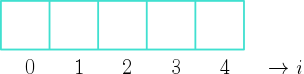
\includegraphics[width=\textwidth]{img/array1D}
    \caption{Logical memory layout representation.}
  \label{fig:1a}
  \end{subfigure}
  \hspace*{4cm}
  \begin{subfigure}[b]{0.25\textwidth}
    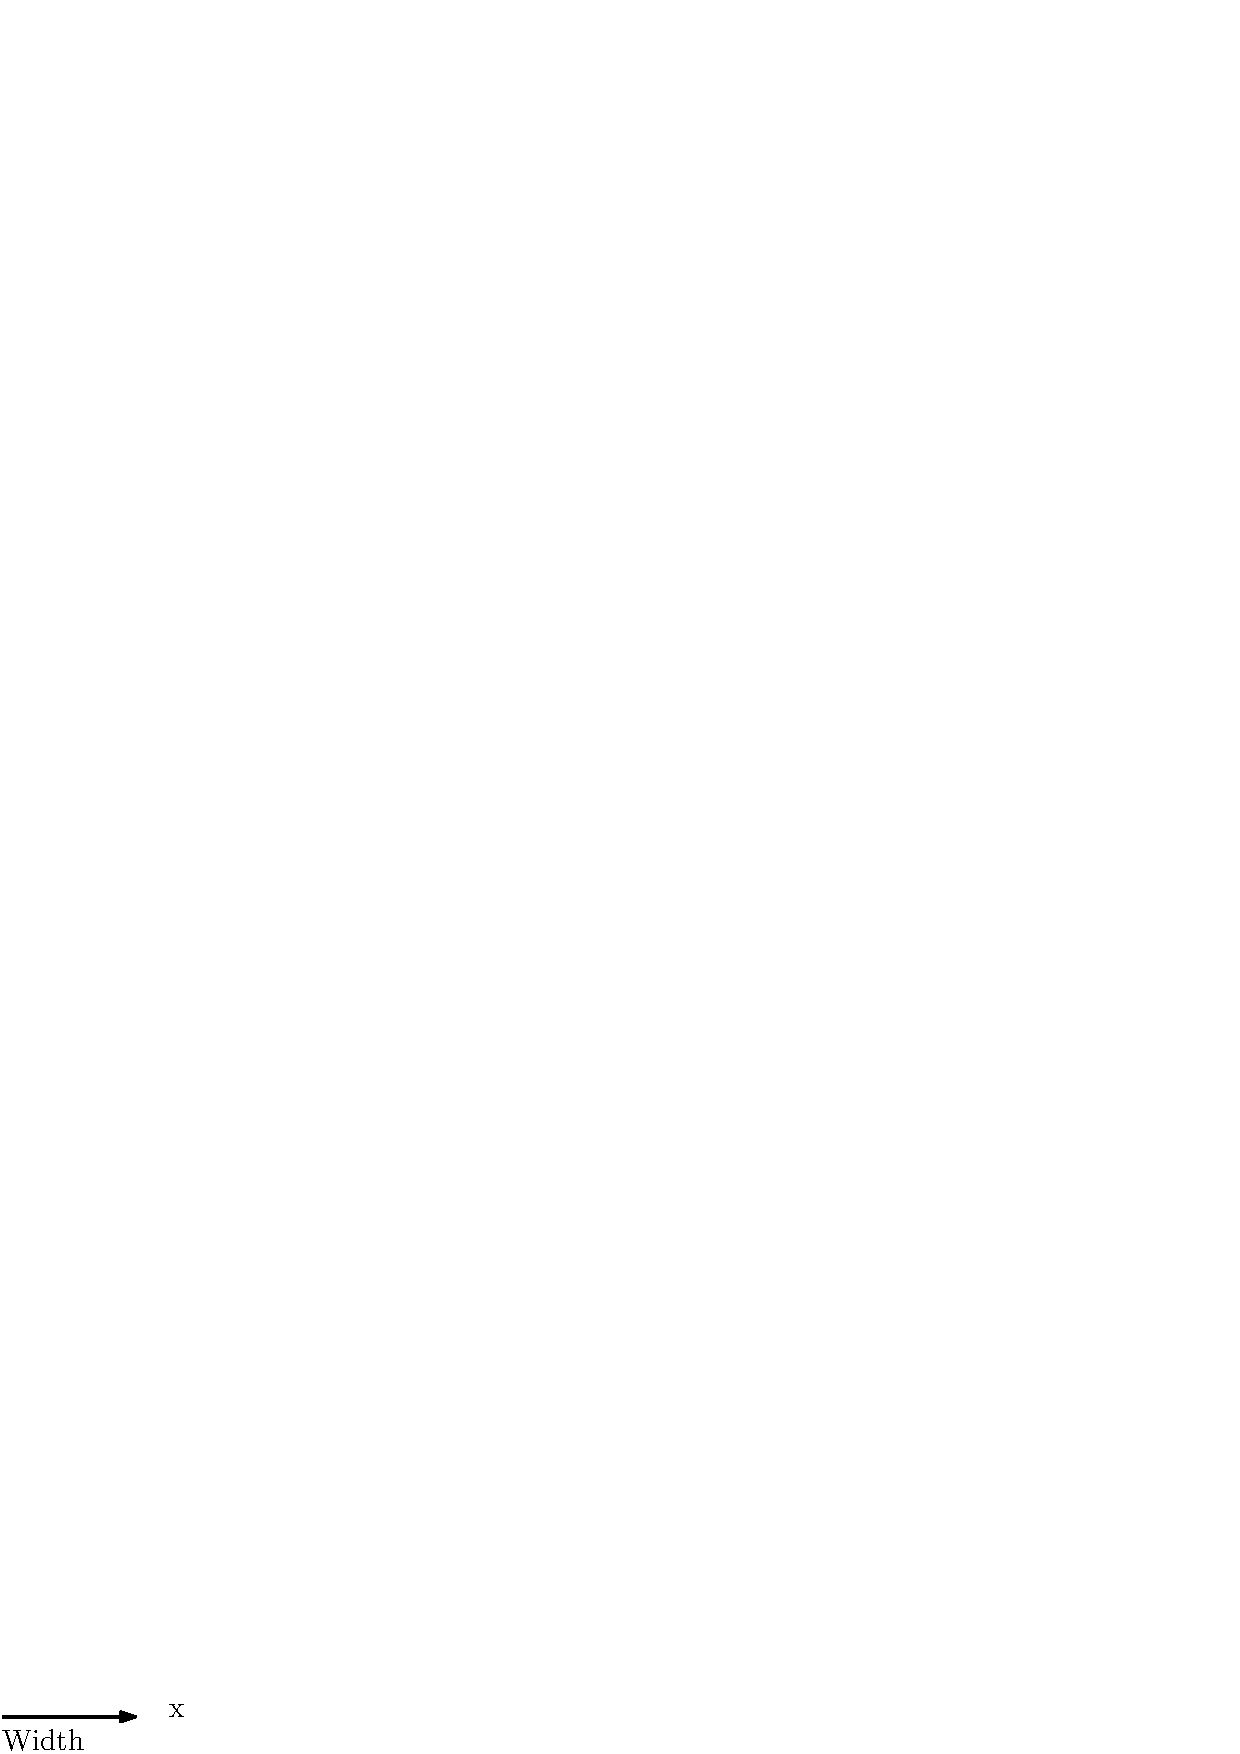
\includegraphics[width=\textwidth]{img/arrow1D}
    \caption{Dimensions represented.}
    \label{fig:1b}
  \end{subfigure}
  \caption{One dimensional array representation.}
  \label{fig:1D}
\end{figure}

\subsection{Two dimensional data}

The problem becomes evident as data start to include more dimensions.
In a bidimensional array we have data that has two dimensions.
One can think about it, like the data it's stored in a table, the situation is the one depicted in Figure~\ref{fig:2a}.
Now, remember this is just an abstraction (provided by our programming language: C++; in this case), since memory is actually \emph{close} to linear in a computer.

\begin{figure}[htp]
  \centering
  \begin{subfigure}[b]{0.35\textwidth}
    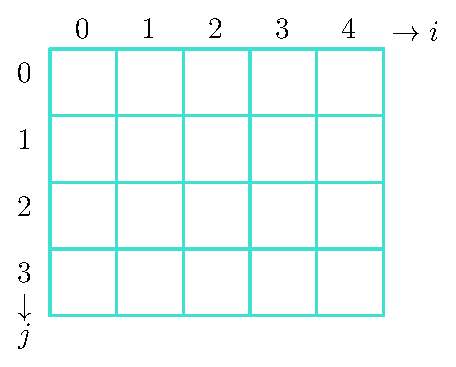
\includegraphics[width=\textwidth]{img/array2D}
    \caption{Logical memory layout representation.}
  \label{fig:2a}
  \end{subfigure}
  \hspace*{4cm}
  \begin{subfigure}[b]{0.25\textwidth}
    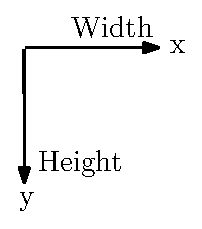
\includegraphics[width=\textwidth]{img/arrow2D}
    \caption{Dimensions represented.}
    \label{fig:2b}
  \end{subfigure}
  \caption{Two dimensional array representation.}
  \label{fig:2D}
\end{figure}

Usually, the C++ way of modeling this is creating an array, such that each element of it, is also an array. See the code in Listing~\ref{lst:2dexample}

{\centering
\begin{minipage}{\linewidth}
  \begin{listing}[H]
  \inputminted[
  xleftmargin=1.5cm,  %without this option line number goes wrong
  %frame=lines,
  framesep=0.5cm,
  baselinestretch=1.2,
  %fontsize=\footnotesize,
  linenos,
  firstline=23, %If you omit this two fields, the whole file is pulled
  lastline=38
  ]{cpp}{src/ArrayDimensions.cpp}
  \caption{Two dimensioal array example}
  \label{lst:2dexample}
  \end{listing}
\end{minipage}
\par
}
\vspace{0.5cm}
Now, there is three main points to highlight in the sample:
\begin{enumerate}

\item The type of the array has change.
      Now is \emph{a vector of int vectors}.
      This led us to have a longer initialization for it too.
      Imagine that you create functions to receive or return such arrays.
      The sintax to declare the parameters will become difficult.

\item We still have the advantage of a very elegant sintax to use the array: \mintinline{cpp}{b[j][i]} give us the element on column $i$ of row $j$.

\item The sintax is backwads with respect to mathematic representation.
      See Figure~\ref{fig:2D} again.
      The index \mintinline{cpp}{i} is transversin along the $x$ dimension and the index \mintinline{cpp}{j} along the $y$ dimension.
      Therefore, the element \mintinline{cpp}{b[j][i]} it's close to $b(x, y)$ in math
 \end{enumerate}

\subsection{Memory flatenig explained}

Here is when the technique called \emph{memory flattening} becomes useful.
In simple words: This is to mimic what the compiler is doing for us: use linear data.
But at the same time you also provide an abstraction, so you can access it in a similar fashion that if your data had more dimensions.
In other works you simulate the access via indices for all the simulated dimensions.

See the Figure~\ref{fig:Flat}.
The data is equivalent to the one shown in Figure~\ref{fig:2D} in the sense that represents a two dimensional table, whose first dimension $x$ (number of columns: $5$), is indexed by $i \in \{0, 1, 2, 3, 4\}$ and whose second dimension $y$ (number of rows: $4$) is indexed by $j \in \{0, 1, 2, 3\}$.
However, the data is stored in a one dimensional array of size $5 \cdot 4 = 20$.
The actual indices of the array $ \in \{ 0, 1, \ldots, 19 \}$ and are shown on the bottom of of Figure~\ref{fig:Flat}.
However, we also provide an abstraction to access this data via simulated indices \mintinline{cpp}{[j][i]} shown in the top of Figure~\ref{fig:Flat}

\begin{figure}[htb]
  \centering
  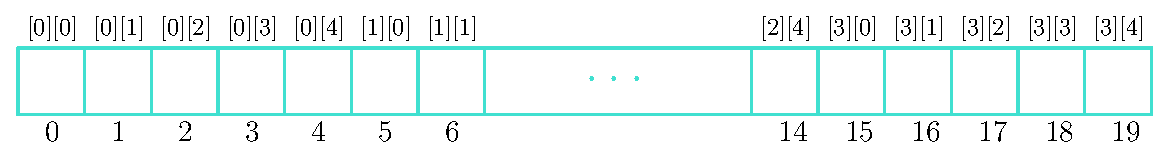
\includegraphics[width=0.85\textwidth]{img/arrayFlat}
  \caption{2D array represented as a \emph{flattened} array. This represents the same data as Figure~\ref{fig:2D}. Order of the indices is \mintinline{cpp}{[j][i]}}
  \label{fig:Flat}
\end{figure}

This has the advantage that all the data is store in a one dimensional array.
Therefore, you \emph{ensure} all your data is actually contigous in memory.
And no matter how many dimensions your data has, the type is always a one dimensional array.

Also, provided that we acces the data in the \emph{correct way}, the access tends to be faster than the alternative shown in Listing~\ref{lst:2dexample}.
The \emph{correct way} means that the inner loop moves along the $x$ dimension and the outer loop transverses the second dimension $y$.
The reason for this improvement becomes evident if we see Figure~\ref{fig:Flat}: in this way, we are actually accesing a linear array in his linear order.

In order to implement this technique we will need two mappings:
First, a function $g:\mathbb{Z}^n \rightarrow \mathbb{Z}$, to map the indices in $n$ dimensions to the one dimensional array.
And second, the inverse mapping $h:\mathbb{Z} \rightarrow \mathbb{Z}^n$ to retrive the indices back given a position in the data buffer.

The first function $g$ it is actually the most useful to us, since it will provide with the interface of accesing our data.
See the Figure~\ref{fig:2D}.
Assume that our data hast two dimensions ($x$ and $y$ --or \emph{width} and \emph{height}-- if you like).
That we use two indices $i$ and $j$ to transverse it.
And assume also that the maximun values of such indices are \mintinline{cpp}{WIDTH} and \mintinline{cpp}{HEIGHT} and that they are zero based.
In Listing~\ref{lst:functions2D} we show the implementation of such function.

We can see that the transformations are actually very simple.
In fact, one of them is the integer division and the other one is the modulo.
Also note, that as long as we check for the boundaries of the values for both indices, only one of the maximun dimensions in this case \emph{witdh} is used in the actual calculation of the indices.

{\centering
\begin{minipage}{\linewidth}
  \begin{listing}[H]
  \inputminted[
  xleftmargin=1.5cm,  %without this option line number goes wrong
  %frame=lines,
  framesep=0.5cm,
  baselinestretch=1.2,
  %fontsize=\footnotesize,
  linenos,
  firstline=88, %If you omit this two fields, the whole file is pulled
  lastline=105
  ]{cpp}{src/FlatMemmory.cpp}
  \caption{Function $g$ to map real index into simulated 2D indices}
  \label{lst:functions2D}
  \end{listing}
\end{minipage}
\par
}
\vspace{0.5cm}

For completeness, we also show Listing~\ref{lst:functions2D2} that defines the inverse function $h$, to retrive the index in the one dimensional array from the two simulated indices in 2D.

{\centering
\begin{minipage}{\linewidth}
  \begin{listing}[H]
  \inputminted[
  xleftmargin=1.5cm,  %without this option line number goes wrong
  %frame=lines,
  framesep=0.5cm,
  baselinestretch=1.2,
  %fontsize=\footnotesize,
  linenos,
  firstline=107, %If you omit this two fields, the whole file is pulled
  lastline=121
  ]{cpp}{src/FlatMemmory.cpp}
  \caption{Function $h$ to map simulated 2D indices into the real index, this is the inverse of $g$}
  \label{lst:functions2D2}
  \end{listing}
\end{minipage}
\par
}
\vspace{0.5cm}

\subsection{Three dimensional data}

Now, lets look at the more complex --but still very common-- scenario of three dimensions. The situation is the one depicted in Figure~\ref{fig:3D}. We include a new dimension in the data: indexed by $k$ along the $z$ axis, we call it \emph{depth}.

\begin{figure}[htp]
  \centering
  \begin{subfigure}[b]{0.35\textwidth}
    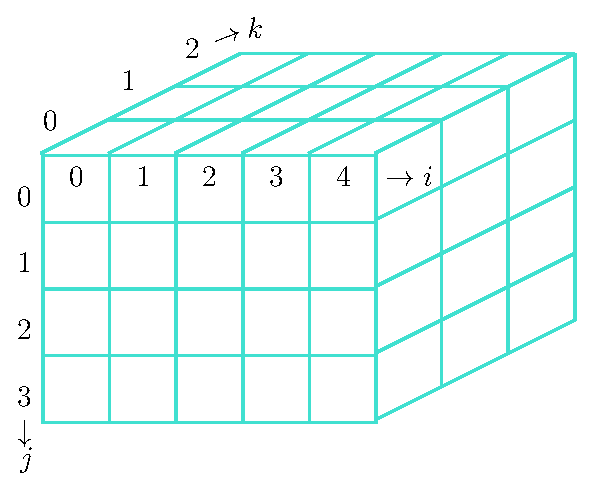
\includegraphics[width=\textwidth]{img/array3D}
    \caption{Logical memory layout representation.}
  \label{fig:3a}
  \end{subfigure}
  \hspace*{4cm}
  \begin{subfigure}[b]{0.2\textwidth}
    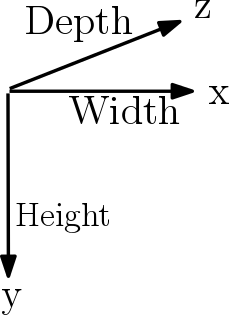
\includegraphics[width=\textwidth]{img/arrow3D}
    \caption{Dimensions represented.}
    \label{fig:3b}
  \end{subfigure}
  \caption{Three dimensional array representation.}
  \label{fig:3D}
\end{figure}

In the normal mutidimensional array synatx C++ syntax this will become, an array of arrays of array of ints. See Listing~\ref{lst:3dexample}. We transvers it using three nested loops, where the most outer one is the one indexed by the new dimension.

{\centering
\begin{minipage}{\linewidth}
  \begin{listing}[H]
  \inputminted[
  xleftmargin=1.5cm,  %without this option line number goes wrong
  %frame=lines,
  framesep=0.5cm,
  baselinestretch=1.2,
  %fontsize=\footnotesize,
  linenos,
  firstline=40, %If you omit this two fields, the whole file is pulled
  lastline=64
  ]{cpp}{src/ArrayDimensions.cpp}
  \caption{Three dimensional array example in C++}
  \label{lst:3dexample}
  \end{listing}
\end{minipage}
\par
}
\vspace{0.5cm}

For memory flatening, we will need a new version of functions $g$ and $h$, that depends in a new extra parameter: \mintinline{cpp}{DEPTH}.
In Listing~\ref{lst:functions3D}, we can see the new function $g$.

{\centering
\begin{minipage}{\linewidth}
  \begin{listing}[H]
  \inputminted[
  xleftmargin=1.5cm,  %without this option line number goes wrong
  %frame=lines,
  framesep=0.5cm,
  baselinestretch=1.2,
  fontsize=\footnotesize,
  linenos,
  firstline=123, %If you omit this two fields, the whole file is pulled
  lastline=143
  ]{cpp}{src/FlatMemmory.cpp}
  \caption{New function $g$ to map real index into simulated 3D indices}
  \label{lst:functions3D}
  \end{listing}
\end{minipage}
\par
}
\vspace{0.5cm}

I will talk about the form of the function for the second parameter (the $y$ that represent the \mintinline{cpp}{j} index) in Section~\ref{sec:moreDim}. Finally, for completenees; the new function $h$ is presented in Listing~\ref{lst:functions3D2}

{\centering
\begin{minipage}{\linewidth}
  \begin{listing}[H]
  \inputminted[
  xleftmargin=1.5cm,  %without this option line number goes wrong
  %frame=lines,
  framesep=0.5cm,
  baselinestretch=1.2,
  fontsize=\footnotesize,
  linenos,
  firstline=145, %If you omit this two fields, the whole file is pulled
  lastline=163
  ]{cpp}{src/FlatMemmory.cpp}
  \caption{A new function $h$ to map simulated 3D indices into the real index, this is the inverse of $g$}
  \label{lst:functions3D2}
  \end{listing}
\end{minipage}
\par
}

\subsubsection{Generalizing to more dimensions}
\label{sec:moreDim}

In the case of two dimensions the calculation for function $g$ were simply the integer division and the modulo. In the case of three dimensions we also have a modulo and a division (Altrought, the parameters change in the later one). However, the interesting case is that of the middle value: it has both operations.

This is actually the general case. Indeed, the correct transformation to get the simulated index of a given dimension, is as follows:
\begin{enumerate}
  \item Divide the real index by the size of the unit of all the previous dimensions.
  \item Take the result of the previous operation and  calculate his modulo with the maximum size of the given dimension.
\end{enumerate}

Let me present an alternative to the function $g$ given in Listing~\ref{lst:functions3D} using the general appproach in Listing~\ref{lst:functions3D3}

{\centering
\begin{minipage}{\linewidth}
  \begin{listing}[H]
  \inputminted[
  xleftmargin=1.5cm,  %without this option line number goes wrong
  %frame=lines,
  framesep=0.5cm,
  baselinestretch=1.2,
  fontsize=\footnotesize,
  linenos,
  firstline=187, %If you omit this two fields, the whole file is pulled
  lastline=205
  ]{cpp}{src/FlatMemmory.cpp}
  \caption{Alternative $g$ function for 3D. Using the general form of the algorithm}
  \label{lst:functions3D3}
  \end{listing}
\end{minipage}
\par
}
\vspace{0.5cm}

Now, it becomes clear why in Listing~\ref{lst:functions3D} we did not need the full forms.
For the $x$ variable the previosu dimension has size one, and we do not need to divide by one.
As for the last index $z$, we know that \mintinline{cpp}{index} is striclly less than \mintinline{cpp}{WIDTH * HEIGHT * DEPTH}, and we divide it by \mintinline{cpp}{WIDTH * HEIGHT}, so it should be a number stricltly less than \mintinline{cpp}{DEPTH}, therefore we do not need to take the modulo.

Now that the the logic of the function $g$ is clear; we can also come up with a general rule for the inverse function $h$.

\begin{enumerate}
  \item For each dimension calculate a term. The term is the size of the unit in the previos dimension times the index in the current dimension.
  \item Accumulate (add) all the terms to calculate the real index.
\end{enumerate}

See Listing~\ref{lst:functions3D4} for the \emph{general rule} implementation.

{\centering
\begin{minipage}{\linewidth}
  \begin{listing}[H]
  \inputminted[
  xleftmargin=1.5cm,  %without this option line number goes wrong
  %frame=lines,
  framesep=0.5cm,
  baselinestretch=1.2,
  fontsize=\footnotesize,
  linenos,
  firstline=166, %If you omit this two fields, the whole file is pulled
  lastline=185
  ]{cpp}{src/FlatMemmory.cpp}
  \caption{Alternative to function $h$ using the general rule}
  \label{lst:functions3D4}
  \end{listing}
\end{minipage}
\par
}

\section{Bit manipulation}
\begin{itemize}
  \item Basic operations. Bit vs Byte How to handle printing in C++
  \item One bit manipulation, set, clear, toggle and testing
  \item Bit masking: set, clear, toggle and test group of bites
\end{itemize}
In this section I will explian some bit manipulation operations. As is common in most programing tasks and to avoid difficult cases; we will foucus on positive values for integer types.

Just to clarify the terms: \emph{bit} is a single binary digit, it can have only two values either 0 or 1. A \emph{byte} is a group of bits that conforms the unit of the computer architecture. Technically, a byte can have any size in bits. However, in modern computers this is always 8. That is why sometimes they call a byte an \emph{octet}. For the following code samples you can assume the following constant to be in scope.

\begin{minted}{cpp}
const size_t BITS_PER_BYTE = 8U;
\end{minted}

Let me introduce, in Listing~\ref{lst:binHelpers}; two helper function to debug and visulize such variables. The first one: \mintinline{cpp}{bitSize} returns the size in bits of the variable and the second one: \mintinline{cpp}{bitStr} returns a string with the binary representation of a variable.

{\centering
\begin{minipage}{\linewidth}
  \begin{listing}[H]
  \inputminted[
  xleftmargin=1.5cm,  %without this option line number goes wrong
  %frame=lines,
  framesep=0.5cm,
  baselinestretch=1.2,
  fontsize=\footnotesize,
  linenos,
  firstline=76, %If you omit this two fields, the whole file is pulled
  lastline=87
  ]{cpp}{src/bitManipulation.cpp}
  \caption{Helper functions to debug bit manipulations}
  \label{lst:binHelpers}
  \end{listing}
\end{minipage}
\par
}

Another important feature in C++ is that we can use both binary (actually since standar C++14) and heaxadecimal literals:
\begin{minted}{cpp}
unsigned char aChar = 0b101010;
int anInt = 0xFF00FF08;
cout << "binary representation of aChar: " << binStr(aChar) << endl;
cout << "binary representation of anInt: " << binStr(anInt) << endl;
\end{minted}
Will print:
\begin{verbatim}
binary representation of aChar: 00101010
binary representation of anInt: 11111111000000001111111100001000
\end{verbatim} 

\subsection{Bit's operations}

The operations that work in bits level are the following:
\begin{itemize}
\item Shift to the left by $n$ bits. Performed with the operator \mintinline{cpp}{<<}.
\item Shift to the right by $n$ bits. Performed with the operator \mintinline{cpp}{>>}.

These binary operations take an integer value (to the left) and an unsigned integer value (to the right) and return the result of an integer value of the same size of the left operand created by shifting the bits of the left operand by the number of bits represented by the right operand.
The bits shifted out are descarted and in order to fill the spaces created by the shift, zeros are inserted.
Because of this, shifting to any side by the exact size in bits of the right operand is the same as setting the result to 0.
However, a quick warning note: Shifting to any side by an number greater than the size (in bits) of the right operand or by a negative number it is not defined. See~\cite{INT34Cpp} for a more detailed explanation.

The code snippet in Listing~\ref{lst:bitShifting} shows a valid C++ sample of these operations:

{\centering
\begin{minipage}{\linewidth}
  \begin{listing}[H]
  \inputminted[
  xleftmargin=1.5cm,  %without this option line number goes wrong
  %frame=lines,
  framesep=0.5cm,
  baselinestretch=1.2,
  fontsize=\footnotesize,
  linenos,
  firstline=36, %If you omit this two fields, the whole file is pulled
  lastline=47
  ]{cpp}{src/bitManipulation.cpp}
  \caption{Sample of bit shiting}
  \label{lst:bitShifting}
  \end{listing}
\end{minipage}
\par
}

Produces the following output:

\begin{verbatim}
a: 00101010 = 42
d: 01010000 = 80
e: 00000101 = 5
f: 00000000 = 0
g: 00000000 = 0
\end{verbatim} 

Another important thing to notice is that, \emph{as long as the shift leaves significant digits} (or else we \emph{underflow}); shifting values to the right is equivalent to divide by $2^n$ where $n$ is the number of bits shifted.
Similarly, shifting values to the left, \emph{as long as we do not discard a significant bit} (or else we \emph{overflow}); is equivalent to multiply by $2^n$, where $n$ is the number of bits shifted.

In the above sample $2^3 = 8$. Therfore: $e = 42 / 8 = 5$ (remember it's an integer division).
And $d = 42 \cdot 8 = 336$, but it resulted in an overflow, since the maximun value for an $8$ bit variable is $2^8 = 256$.

\item Bitwise \emph{AND} between two values of the same size. Performed with the operator \mintinline{cpp}{&}. Yes, it is the same as the \emph{dereference} operator. The distinctions is made due the former being a binary operator and the dereference one being a unary operator.
\item Bitwise \emph{OR} between two values of the same size. Performed with the operator \mintinline{cpp}{|}
\item Bitwise \emph{XOR} between two values of the same size. Also known as \emph{exclusive or}. Performed with the operator \mintinline{cpp}{^}

These operators are the expected equivalent to the ones defined in first order logic.
However, they operate bitwise; that is why they are different than the logical ones that are represented by double ampersand or double pipe.

\item Bitwise unary \emph{NOT}. Performed with the operator \mintinline{cpp}{~}
\end{itemize}

Listing~\ref{lst:bitwiseOp} present a sample usage of the bitwise logical operations:

{\centering
\begin{minipage}{\linewidth}
  \begin{listing}[H]
  \inputminted[
  xleftmargin=1.5cm,  %without this option line number goes wrong
  %frame=lines,
  framesep=0.5cm,
  baselinestretch=1.2,
  fontsize=\footnotesize,
  linenos,
  firstline=50, %If you omit this two fields, the whole file is pulled
  lastline=71
  ]{cpp}{src/bitManipulation.cpp}
  \caption{Bitwise operations sample}
  \label{lst:bitwiseOp}
  \end{listing}
\end{minipage}
\par
}

And produces the following result:

\begin{verbatim}
c = a & b
a: 10101101
b: 11100110
c: 10100100
d = a | b
a: 10101101
b: 11100110
d: 11101111
e = a ^ b
a: 10101101
b: 11100110
e: 01001011
f = ~a
a: 10101101
f: 01010010
\end{verbatim}

\subsection{Bit manipulations}

In order to do bit manipulations, we need to be able to refer to a specific bit.
The bits on a variable are refered by a position.
The first position, is the leftmost bit; its refered as $0$ and contunie to increment to the right until the last bit.
Look at the Figure~\ref{fig:bitPos}
Therefore, in an $8$ bit size variable positions are in $\{ 0, 1, \ldots, 6, 7 \}$ and in a $32$ bit variable are in $\{ 0, 1, \ldots, 30, 31 \}$.

\begin{figure}[htb]
  \centering
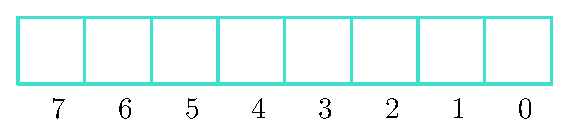
\includegraphics[width=0.85\textwidth]{img/bitPositions}
  \caption{Positions of the bits in a variable.}
  \label{fig:bitPos}
\end{figure}

Extra note: \emph{endianism does not matter for bit manipulations}.
The languaje (in this case C++) abstract this for you.
Endianism only matter when you are reading or writing to the filesystem.
So, for the purposes of this explanation: all machines are big endian.

There are four important operations for bit manipulation:
\begin{description}
\item[Set] Put in an specific bit to the value of $1$.
\item[Unset] Put in an specific bit to the value of $0$.  
\item[Toggle] Change the value of a specific bit. In other words if bit is $1$ set it to $0$. If the bit is $0$ set it to $1$.
\item[Query] This operation results in a boolean value. If an specif bit is $1$ return \mintinline{cpp}{true}, else return \mintinline{cpp}{false}.
\end{description}

In order to implement the bit manipulation we have to use the bit operations in combination with what is called a \emph{mask}.
A mask is another variable of the same size of the one we want to manipulate, that only contain ones in the places we want to manipulate.
Technically, a mask could be of any size, but the explanation get easier if you imagine them of the same size.

As an example, lets construct an $8$ bit mask for manipulating the bit at position $3$.
\begin{itemize}
 \item We start with the value of $1$, in binary representation: $00000001$.
 \item Now, we shift to the left by $n$ bits. Where $n$ is the desired position.
 \item In other words to construct the mas we could do: \mintinline{cpp}{1 << 3}.
 \item The mask is: $00001000$
\end{itemize}


\section{Analytic Geometry}
\begin{itemize}
  \item Ray, line and segment representations
  \item Ray to segment intersection
  \item Projecction
  \item Point to segment distance
  \item Belonging test on simple polygons
\end{itemize}

\section{Graphics Pipeline}
\begin{itemize}
  \item Simple: Vertex and fragment
  \item Complete, all optional stages
  \item Texture pipeline
\end{itemize}
